\documentclass[border=10pt]{standalone}
\usepackage{xcolor}
\usepackage{pgf}
\usepackage{tikz}
\usetikzlibrary{arrows.meta}

\usetikzlibrary{arrows}
\usetikzlibrary{calc}
\usetikzlibrary{shapes}
\usetikzlibrary{trees}
\tikzset{>=stealth'}

% for pic 3
\usetikzlibrary{decorations.pathreplacing,calligraphy}

\newcommand{\blue}{\color{blue}}
\newcommand{\black}{\color{black}}

\begin{document}


%pic 3
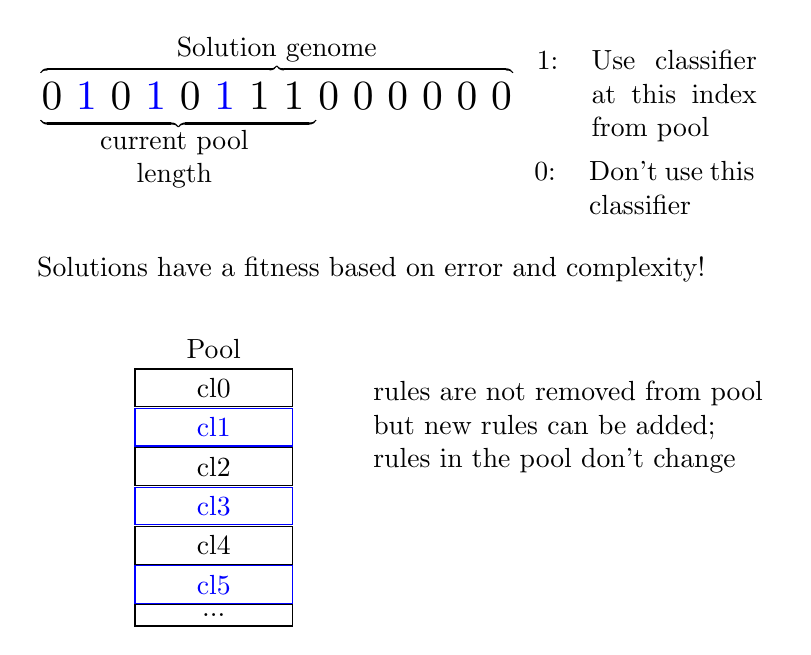
\begin{tikzpicture}[every node/.style={draw=none,minimum width=2cm,align=center}]

\draw node at (0,0.6) (sg) {Solution genome};
\draw node[scale=1.5] at (0,0) (bin) {0 \blue 1 \black 0  \blue 1 \black 0 \blue 1 \black 1 1 0 0 0 0 0 0};
\draw node at (-1.3,-0.8) (p) {current pool\\ length};
\draw [decorate,thick,decoration = {calligraphic brace}] (-3,0.3) --  (3,0.3);
\draw [decorate,thick,decoration = {calligraphic brace}] (0.5,-0.3) --  (-3,-0.3);

\draw node[right of=bin,xshift=3.7cm,align=left] (one) {\begin{tabular}{cp{2.1cm}}
1: & Use classifier at this index from pool \\
\end{tabular}};
\draw node[below of=one,xshift=-0.03cm,yshift=-0.2cm,align=left] (zero) {\begin{tabular}{cp{2.1cm}}0: & Don't use this classifier\end{tabular}};

\draw node[below of=p,xshift=2.5cm,yshift=-0.4cm,align=left] (s) {Solutions have a fitness based on error and complexity!};

\draw node[below of=s,xshift=-2cm] (pool) {Pool};
\draw node[draw=black,rectangle,below of=pool,minimum width=2cm,yshift=0.5cm] (cla) {cl0};
\draw node[draw=blue,rectangle,minimum width=2cm,below of=cla,yshift=0.5cm] (clb) {\blue cl1};
\draw node[draw=black,rectangle,minimum width=2cm,below of=clb,yshift=0.5cm] (clc) {cl2};
\draw node[draw=blue,rectangle,minimum width=2cm,below of=clc,yshift=0.5cm] (cld) {\blue cl3};
\draw node[draw=black,rectangle,minimum width=2cm,below of=cld,yshift=0.5cm] (cle) {cl4};
\draw node[draw=blue,rectangle,minimum width=2cm,below of=cle,yshift=0.5cm] (clf) {\blue cl5};
\draw node[draw=black,rectangle,minimum width=2cm,below of=clf,yshift=0.61cm] (clx) {...};

\draw node[right of=pool,xshift=3.5cm,yshift=-1cm,align=left] (rules) {rules are not removed from pool\\ but new rules can be added;\\ rules in the pool don't change};

\end{tikzpicture}



\end{document}

